%===============================================
\section{Measurement of Higgs boson couplings}
\frame{\tableofcontents[currentsection]}

%%=================================================================================
\begin{frame}{Simplified Template Cross (X) Section (STXS) framework}
  \centering
      \begin{tikzpicture}
      \node[anchor=south west] {\includegraphics[width=0.8\linewidth]{HTSX.pdf}};
%      \draw[step=1.0,black,thin] (0,0) grid (9,7);
      \draw[red, line width=0.5mm, rounded corners =2pt] ( 8.5, 5.2 ) rectangle (9.73, 6.26 ) ;
    \end{tikzpicture}
      
      Cross-sections in exclusive phase space regions (truth bins) allows to measure \textcolor{red}{signal strengths ($\mu=\frac{\sigma^{exp}}{\sigma^{th}}$)}.
  
\end{frame}
%%=================================================================================
\begin{frame}{Couplings measurement strategy}

  \begin{minipage}{0.49\linewidth}
  {\bf Inclusive selection }
  \begin{itemize}
  \item 2 tight isolated photons
  \item $\frac{p_T^{\gamma_{1(2)}}}{m_{\gamma\gamma}} > 0.35~ (0.25)$
  \item $|\eta|\in [0, 1.37]  \cup [1.52, 2.37]$
  \item $m_{\gamma\gamma} \in [105, 160]$ GeV
  \end{itemize}
  \end{minipage}
  \hfill
  \begin{minipage}{0.49\linewidth}
    {\bf Dataset properties}  

    \begin{itemize}
    \item $\sim$ 330k events
    \item $42\%$ signal efficiency
    \item $\simeq 1730$ SM expected signal yield
    \end{itemize}
  \end{minipage}
  \vfill
  {\bf Analysis strategy } 
  \begin{itemize}
  \item Define reconstructed categories targetting specific truth bin.
  \item Measure acceptance of each category wrt truth bins.
  \item Evaluate systematics effects on signal model.
  \item Combined fit of $m_{\gamma\gamma}$ distribution with signal+bkg model.
  \end{itemize}

\end{frame}

%%=================================================================================
\begin{frame}{Reconstructed categories}
  \begin{minipage}{0.49\linewidth}
      \includegraphics[width=\linewidth]{ATL-COM-PHYS-2016-1784_flowchart-eps-converted-to.pdf}
  \end{minipage}
  \hfill
  \begin{minipage}{0.49\linewidth}
    Optimised sensitivity to :
    \begin{itemize}
    \item rare processes
    \item truth bins
    \item detector resolution
    \end{itemize}
%    \includegraphics[width=\linewidth]{ATLAS-CONF-2017-045_4t.pdf}
  \end{minipage}
\end{frame}

%%=================================================================================
\begin{frame}{Signal events distribution over truth bins per category}
  \begin{minipage}{0.6\linewidth}
      \includegraphics[width=\linewidth]{ATL-COM_PHYS_2016-1784_purity_2D.pdf}
  \end{minipage}
  \hfill
  \begin{minipage}{0.39\linewidth}
    \begin{itemize}
    \item \textcolor{blue}{Columns : distribution of events of a given category over the truth bins.}
    \item Rectangles : process optimised categories
    \end{itemize}
  \end{minipage}
  
  \centering
  \textcolor{red}{\bf Good performances of process targetting}
\end{frame}
%%=================================================================================
\begin{frame}{Calibration uncertainties methodology}

      For each systematic sources (energy scale for example) and each category : 
      \begin{itemize}
      \item Create distributions of :
        \begin{itemize}
        \item $m^\text{nom} = m^{rec}\sqrt{(1+\alpha_1)(1+\alpha_2)}$
        \item \textcolor{red}{$m^\text{up} = m^{rec}\sqrt{(1+\alpha_1 + \Delta\alpha_1)(1+\alpha_2+\Delta\alpha_2)}$}
        \item \textcolor{green}{$m^\text{down} = m^{rec}\sqrt{(1+\alpha_1 - \Delta\alpha_1)(1+\alpha_2-\Delta\alpha_2)} $}
        \end{itemize}

      \end{itemize}

  \begin{minipage}{0.49\linewidth}
    \begin{itemize}
            \item Fit distributions using signal model (Double Sided Crystal Ball)
    \item Define systematic variation : \\$\Delta X = \frac{X^{fluct}}{X^{nom}}-1$ \\ $X\in {\text{mean, RMS, yield}}$
    \end{itemize}
    \end{minipage}
    \hfill
    \begin{minipage}{0.49\linewidth}
      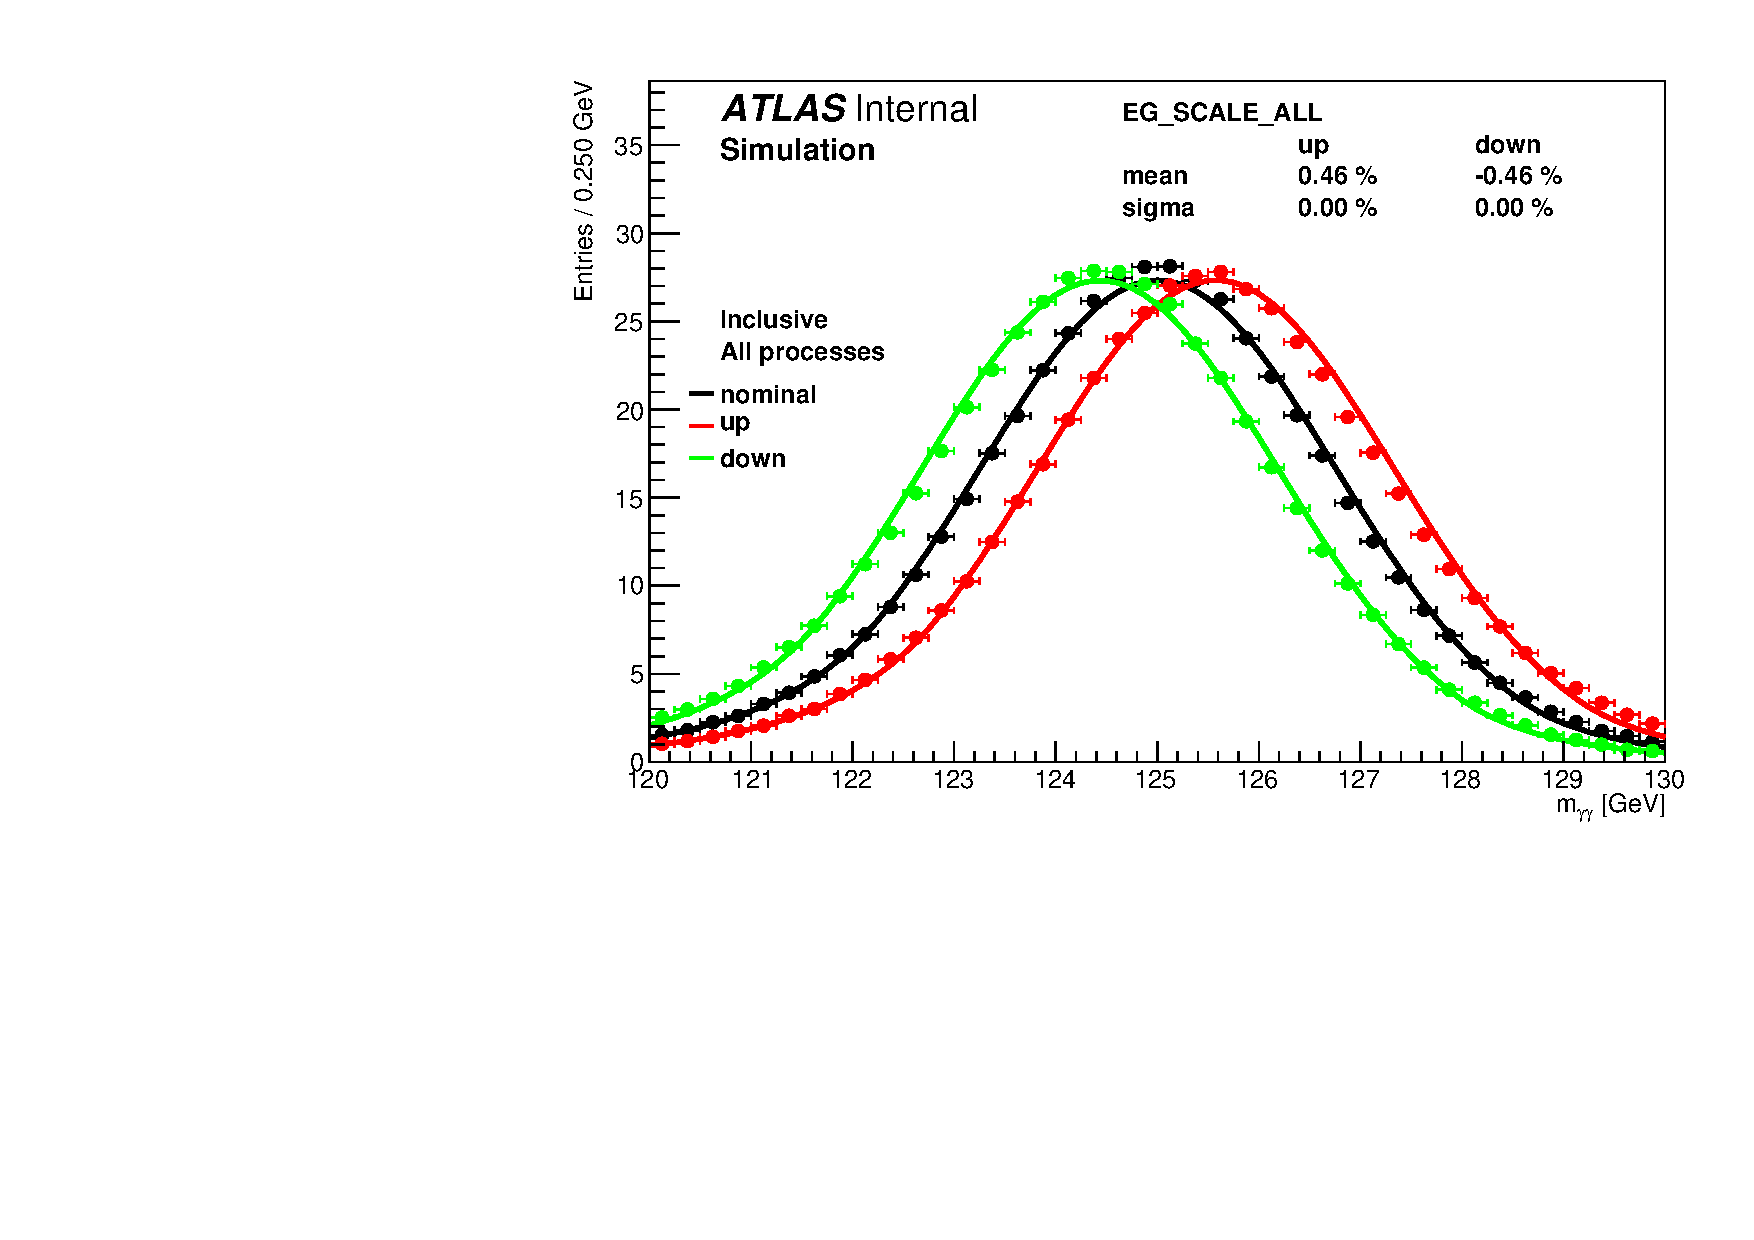
\includegraphics[width=\linewidth]{Figures/h013_EG_SCALE_ALL_0.pdf}
    \end{minipage}
    \vfill
      1 source of uncertainty = 1 nuisance parameter (NP)
\end{frame}

%=================================================================================
\begin{frame}{Correlation models }
  \begin{center}{\bf Two correlation models : } \end{center}
  \begin{minipage}[t]{0.49\linewidth}
    {\bf 1NP }
    \begin{itemize}
    \item 2NP (scale + resolution)
    \item Fully correlated
    \item Conservative
    \item Faster
    \end{itemize}
  \end{minipage}
  \hfill
  \begin{minipage}[t]{0.49\linewidth}
    {\bf FULL}
    \begin{itemize}
    \item 86 NP (77 scale + 9 resolution)
    \item True correlation
    \end{itemize}
  \end{minipage}
  
  \begin{minipage}{0.49\linewidth}
    \resizebox{\linewidth}{!}{
      \begin{tabular}{l|ll}
        Total Scale Uncertainty (\%) & 1NP & FULL \\
        \hline
        Measurement with $H\rightarrow\gamma\gamma$ MC & 0.46 & 0.27\\
        Formula & 0.47 & 0.26\\
      \end{tabular}
    }
  \end{minipage}
  \hfill
  \begin{minipage}{0.49\linewidth}
    \includegraphics[width=\linewidth]{CompareFULLMerge_mean_InclusiveUp.pdf}
  \end{minipage}

\end{frame}
%=================================================================================
\begin{frame}{Calibration uncertainties results}

  \begin{minipage}{0.49\linewidth}
    \centering
    {\bf Merged Model : 49 NP }
    \begin{itemize}
    \item 9 for resolution
    \item 40 for scale
    \end{itemize}
    \vfill
    {\bf impacting }
    \begin{itemize}
    \item resolution
    \item mass
    \item yield per category
      \end{itemize}
  \end{minipage}
  \hfill
  \begin{minipage}{0.49\linewidth}
    \begin{tikzpicture}
      \node[anchor=south west] {    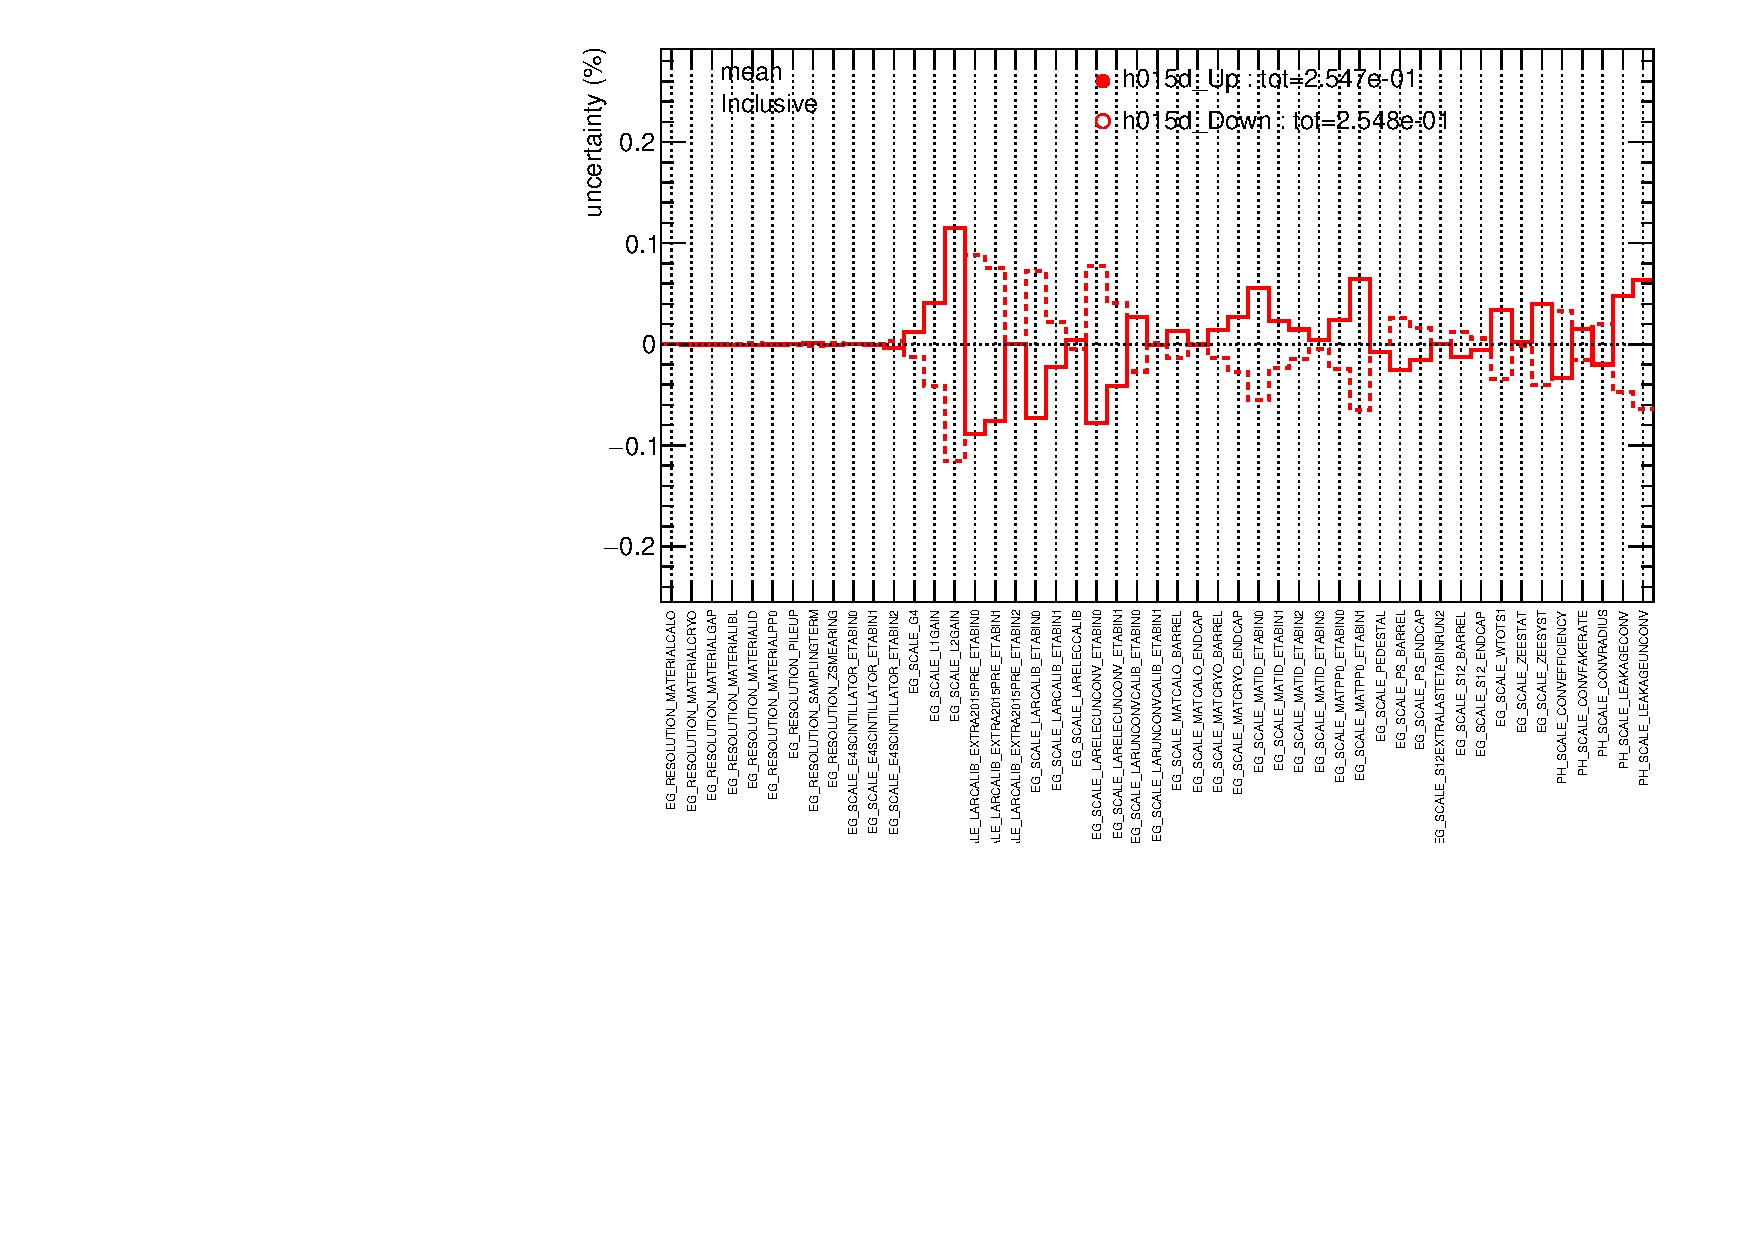
\includegraphics[width=\linewidth]{Figures/h015d_FULLMerge_catMerge_Systematics_Inclusive_mean_mean.pdf}};
      \node[draw] at (2.2,3.88) {mean};
    \end{tikzpicture}
  \end{minipage}

  \begin{minipage}{0.49\linewidth}
    \begin{tikzpicture}
      \node[anchor=south west] {    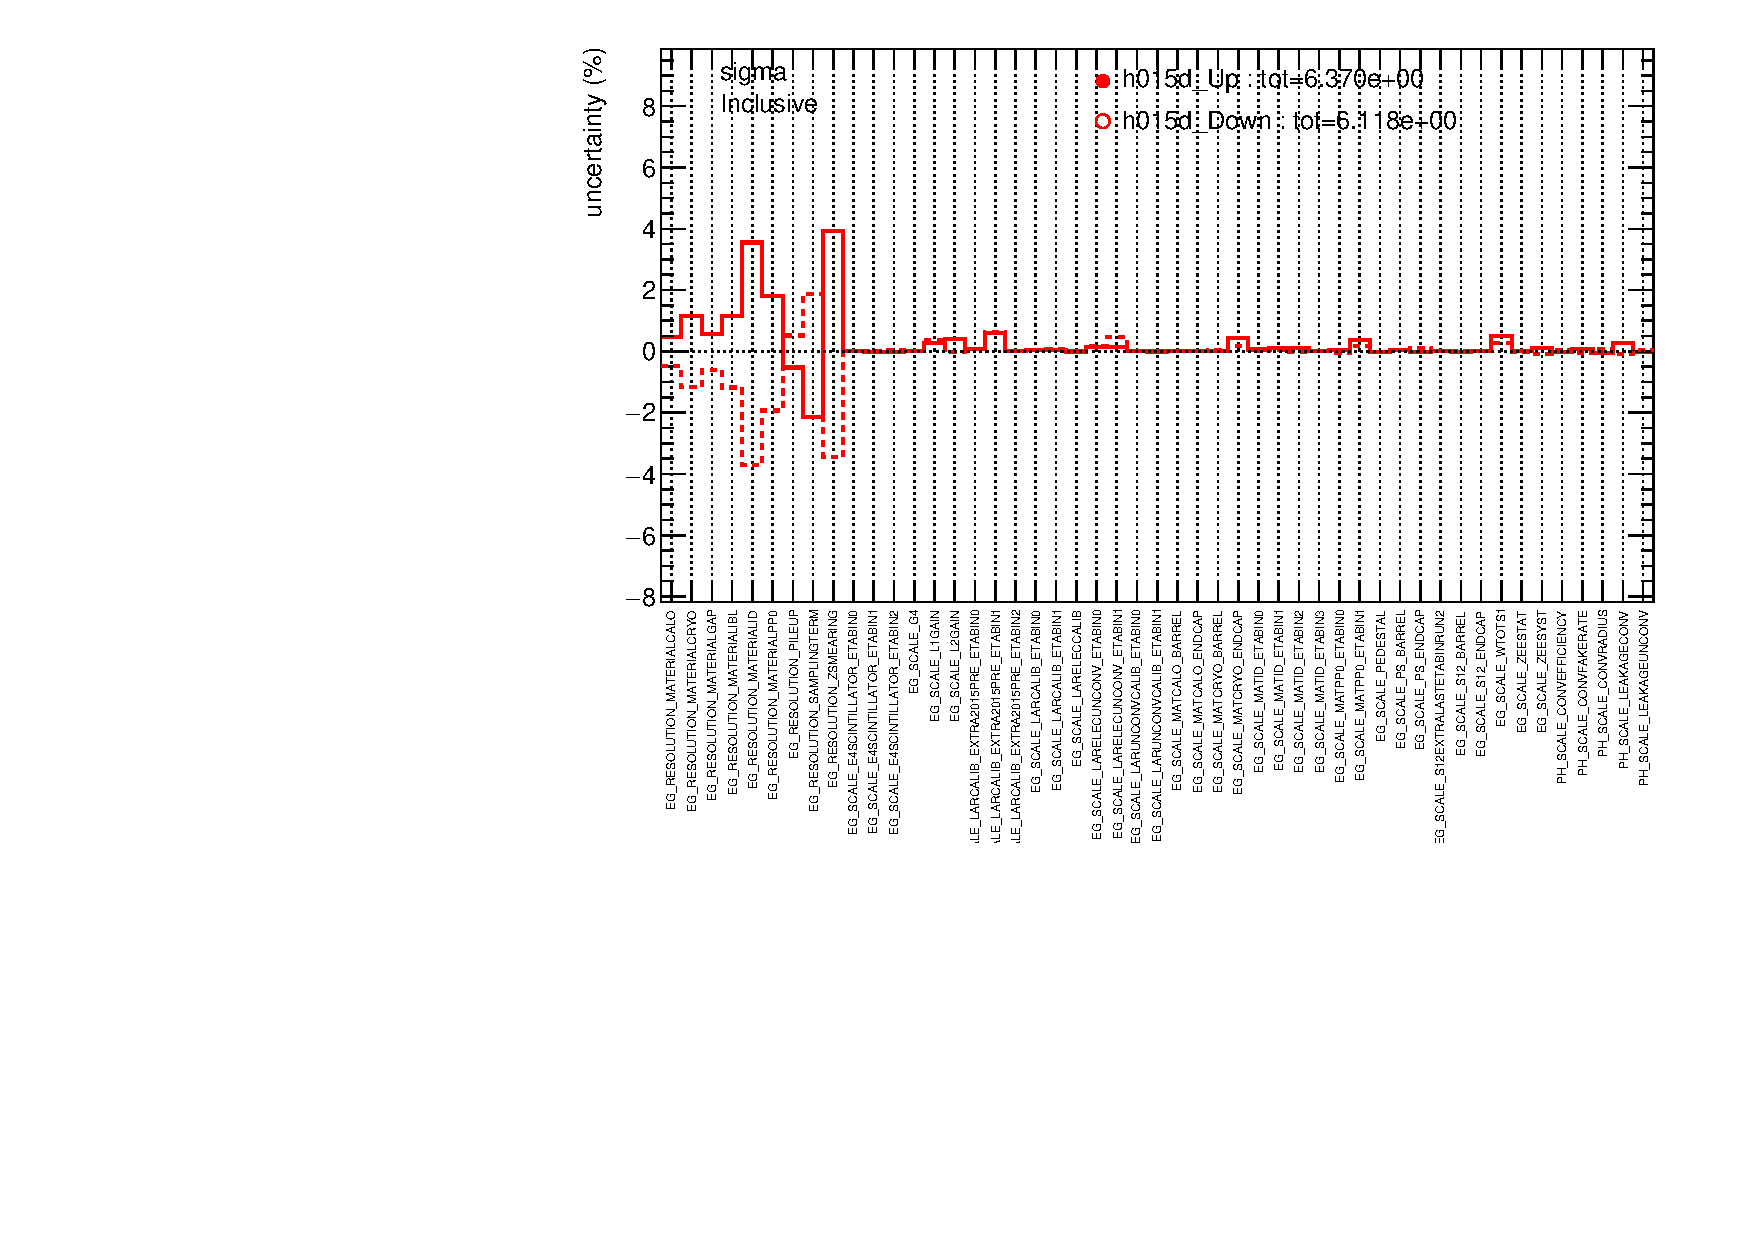
\includegraphics[width=\linewidth]{Figures/h015d_FULLMerge_catMerge_Systematics_Inclusive_sigma_sigma.pdf}};
      \node[draw] at (2.2,3.82) {RMS};
    \end{tikzpicture}
  \end{minipage}
  \hfill
  \begin{minipage}{0.49\linewidth}
    \begin{tikzpicture}
      \node[anchor=south west] {    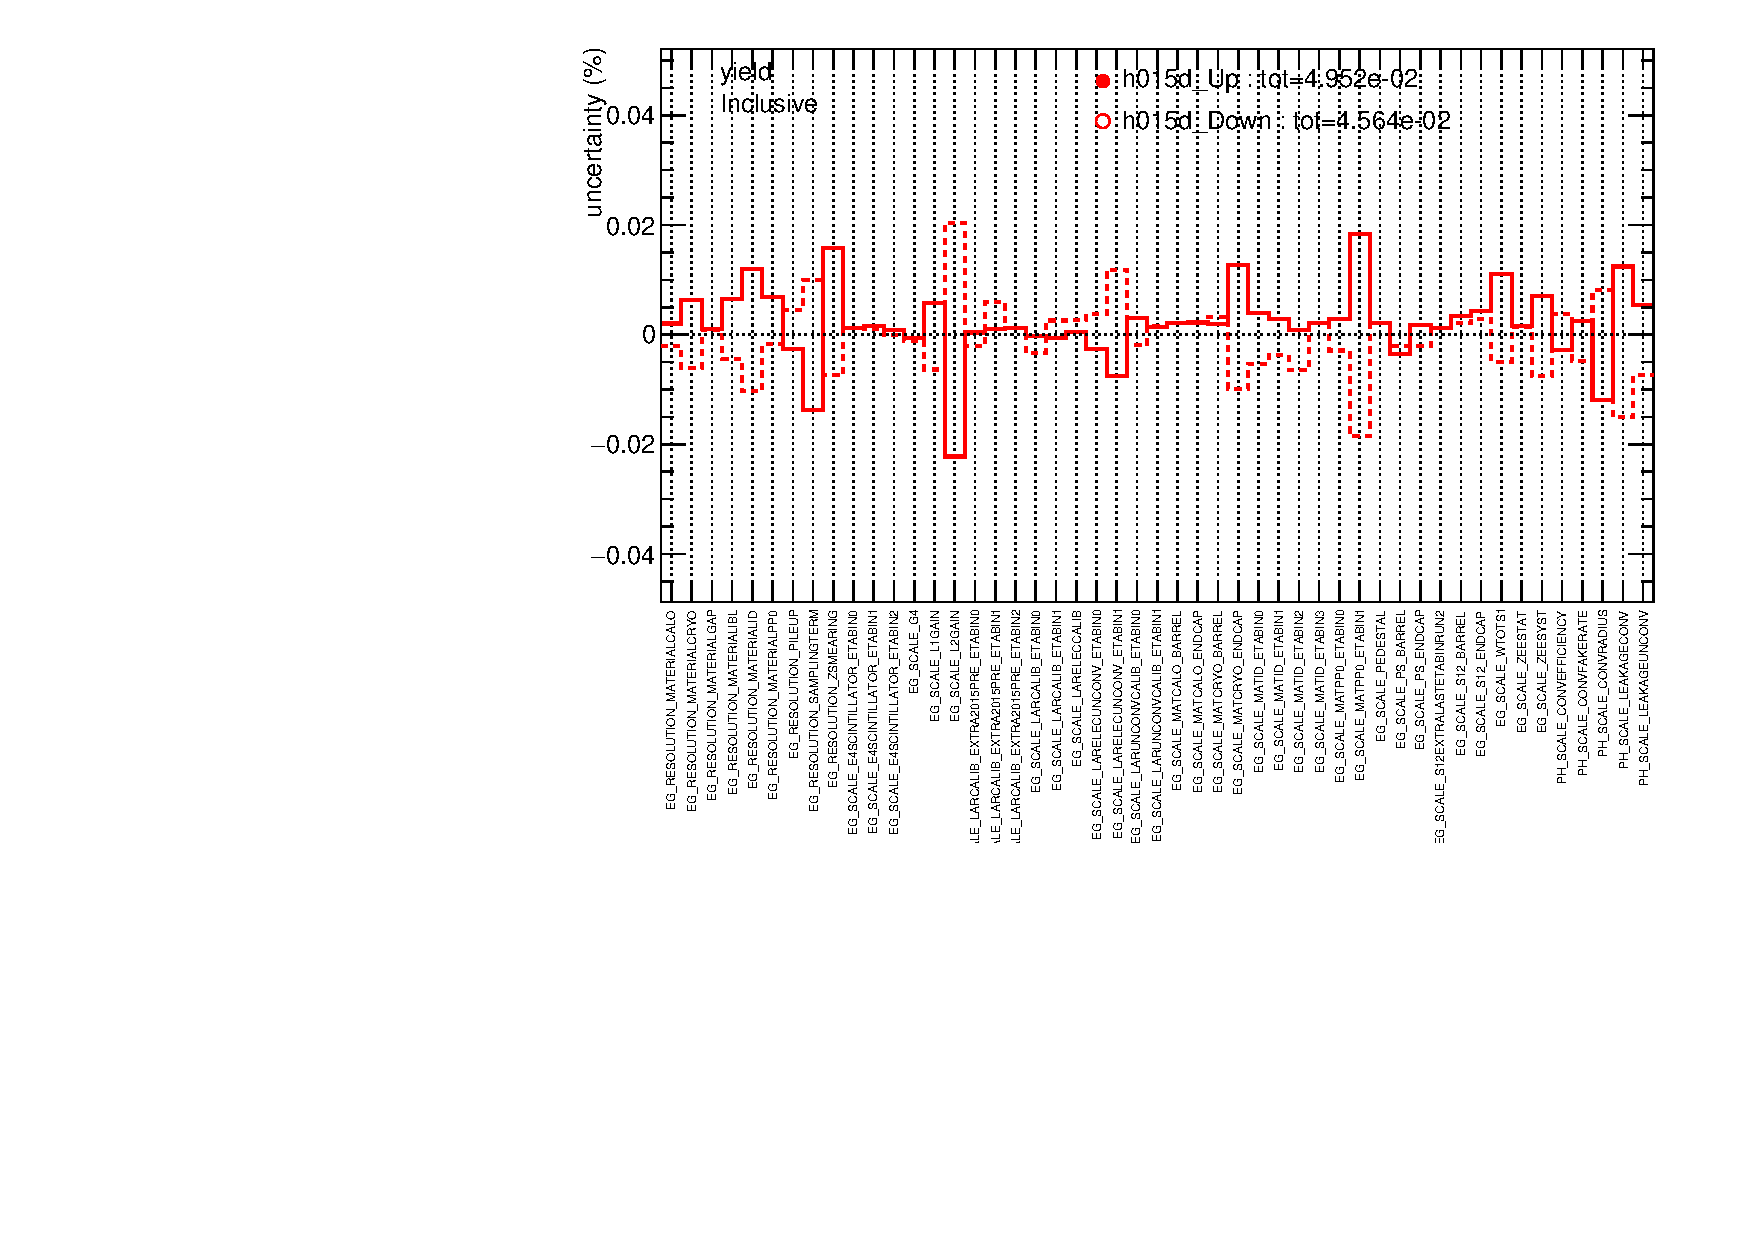
\includegraphics[width=\linewidth]{Figures/h015d_FULLMerge_catMerge_Systematics_Inclusive_yield_yield.pdf}};
      \node[draw] at (2.2, 3.8) {yield};
    \end{tikzpicture}
  \end{minipage}

\end{frame}
%%=================================================================================
\begin{frame}{Total uncertainty}
  \centering
  Total calibration uncertainty as a function of reconstructed category.\\
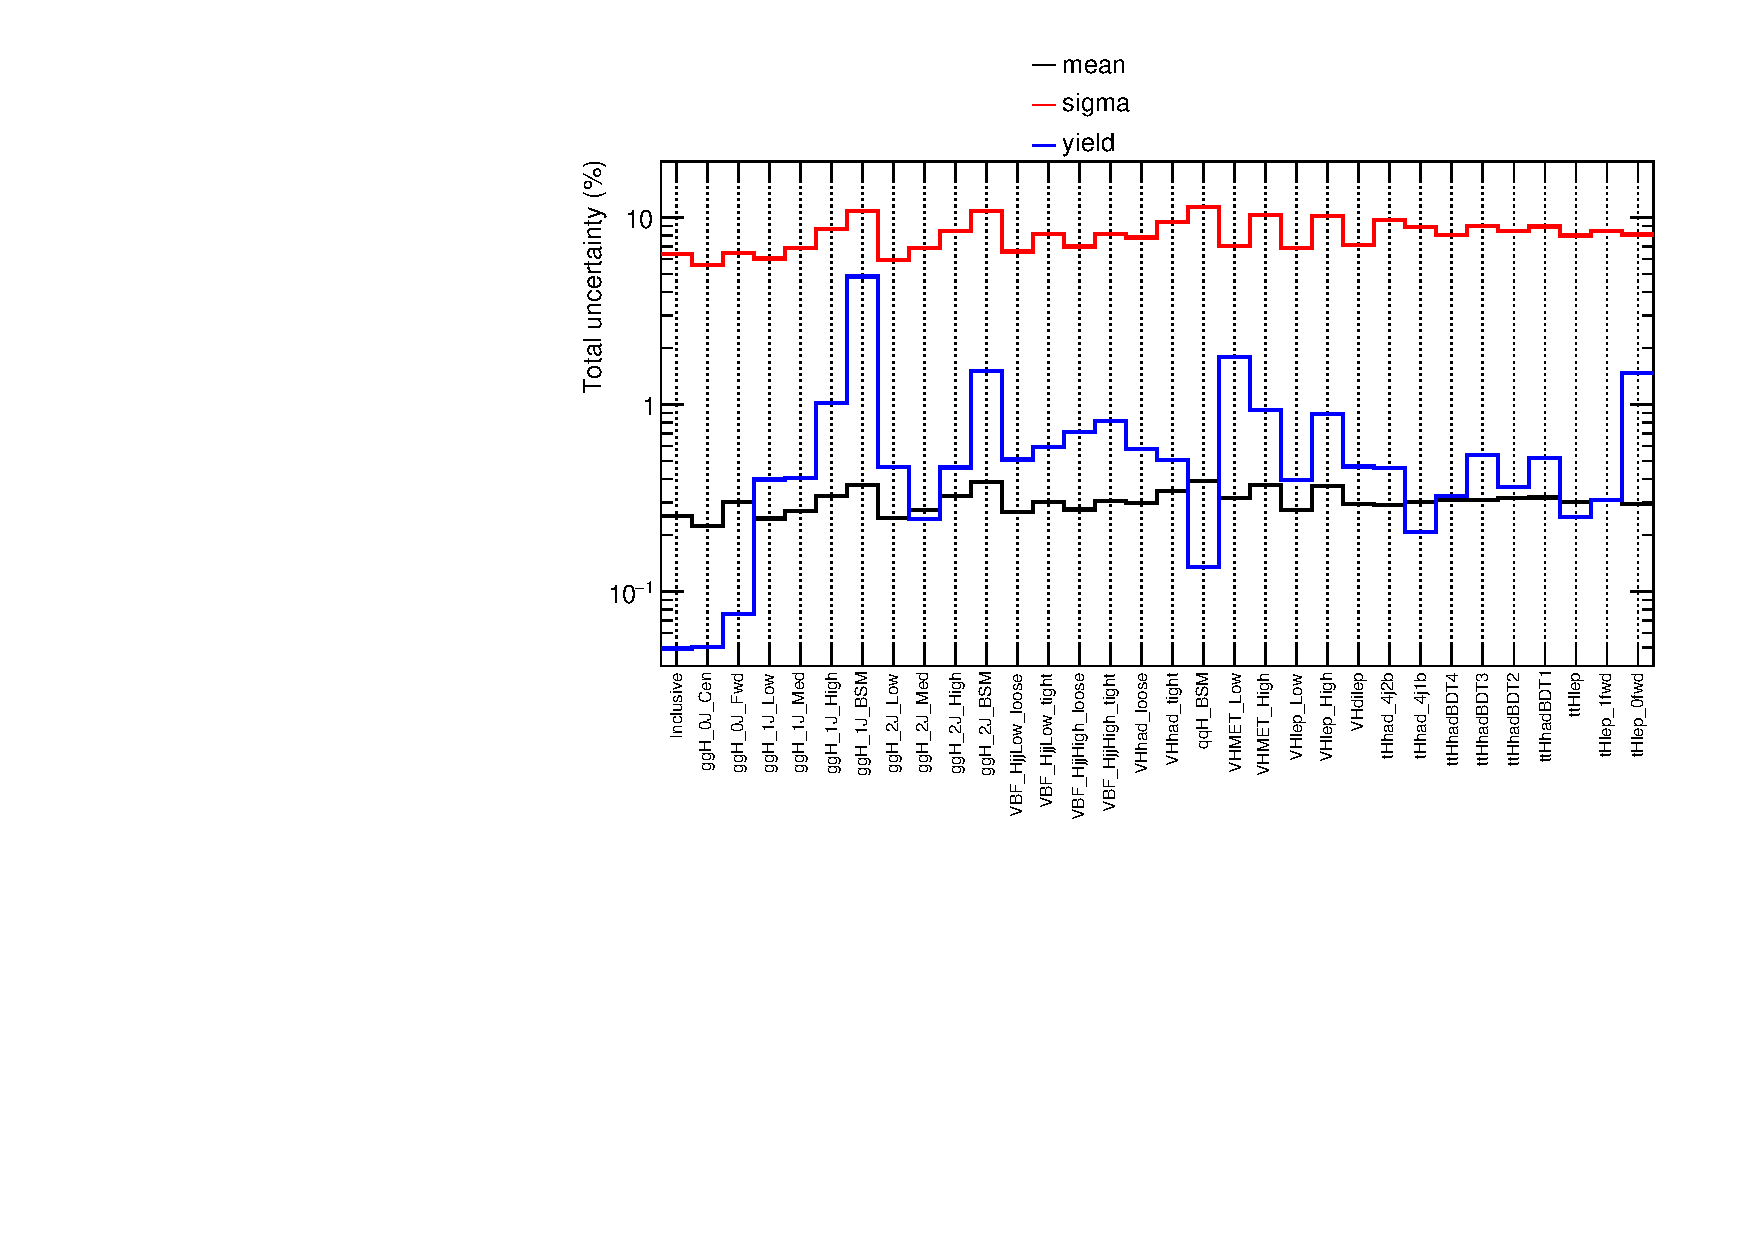
\includegraphics[width=0.9\linewidth]{Figures/h015d_FULLMerge_catMerge_Systematics_InclusiveUp.pdf}  
\end{frame}
%%=================================================================================

\begin{frame}{Run 2 $H\rightarrow \gamma\gamma$  couplings results}
  \centering
  Due to lack of statistics, some truth bins have been merged.
  Grey area represents theory uncertainty (not included in measurement).

  \includegraphics[width=0.55\linewidth]{ATLAS-CONF-2017-045_15f.pdf}
%%   \tiny 
%%   \begin{align*}
%%     \sigma (ggH, \mathrm{0~jet}) \tbfhyy &= 63\ ^{+17}_{-16}\ \fb  &= 63\ ^{+15}_{-15}\,\mathrm{(stat.)}\ ^{+8}_{-6}\,\mathrm{(syst.)}\ \fb \\
%%     \sigma (ggH, \mathrm{1~jet}, p_T^{H} < 60\ \text{GeV}) \tbfhyy &= 15\ ^{+13}_{-12}\ \fb  &= 15\ ^{+12}_{-12}\,\mathrm{(stat.)}\ ^{+6}_{-4}\,\mathrm{(syst.)}\ \fb \\
%%     \sigma (ggH, \mathrm{1~jet}, 60 \leq p_T^{H} < 120\ \text{GeV}) \tbfhyy &= 10\ ^{+7}_{-6}\ \fb  &= 10\ ^{+6}_{-6}\,\mathrm{(stat.)}\ ^{+2}_{-1}\,\mathrm{(syst.)}\ \fb \\
%%     \sigma (ggH, \mathrm{1~jet}, 120 \leq p_T^{H} < 200\ \text{GeV}) \tbfhyy &= 1.7\ ^{+1.7}_{-1.6}\ \fb  & = 1.7\ ^{+1.6}_{-1.6}\,\mathrm{(stat.)}\ ^{+0.6}_{-0.4}\,\mathrm{(syst.)}\ \fb \\
%%     \sigma (ggH, \geq 2~\mathrm{jet}) \tbfhyy &= 11\ ^{+8}_{-8}\ \fb  &= 11\ ^{+8}_{-8}\,\mathrm{(stat.)}\ ^{+3}_{-2}\,\mathrm{(syst.)}\ \fb \\
%%     \sigma (qq \rightarrow Hqq, p_T^{j} < 200~\text{GeV}) \tbfhyy &= 10\ ^{+6}_{-5}\ \fb  &= 10\ ^{+5}_{-5}\,\mathrm{(stat.)}\ ^{+2}_{-1}\,\mathrm{(syst.)}\ \fb \\
%%     \sigma (ggH + qq \rightarrow Hqq, \mathrm{BSM-like}) \tbfhyy &= 1.8\ ^{+1.4}_{-1.4}\ \fb  &= 1.8\ ^{+1.3}_{-1.3}\,\mathrm{(stat.)}\ ^{+0.5}_{-0.5}\,\mathrm{(syst.)}\ \fb \\
%%     \sigma (\mathrm{VH, leptonic}) \tbfhyy &= 1.4\ ^{+1.4}_{-1.2}\ \fb  &= 1.4\ ^{+1.3}_{-1.2}\,\mathrm{(stat.)}\ ^{+0.3}_{-0.3}\,\mathrm{(syst.)}\ \fb \\
%%     \sigma (\mathrm{top}) \tbfhyy &= 1.3\ ^{+0.9}_{-0.8}\ \fb  &= 1.3\ ^{+0.9}_{-0.8}\,\mathrm{(stat.)}\ ^{+0.3}_{-0.1}\,\mathrm{(syst.)}\ \fb \\
%% \end{align*}

\end{frame}
%%====================================================================
\begin{frame}{Run 2 $H\rightarrow \gamma\gamma$ signal strength results}
  STXS difficult to interpret directly.\\
  Measurement of signal strengths $\mu_i = \frac{\sigma_i^{exp}}{\sigma_i^{SM}}$  performed ($\mu=1=\text{SM}$).\\

  \begin{minipage}{0.49\linewidth}
    \includegraphics[width=\linewidth]{ATLAS-CONF-2017-045_11f.pdf}
  \end{minipage}
  \hfill
  \begin{minipage}{0.49\linewidth}
    \centering
    \begin{tikzpicture}
      \node[anchor=south west] {    \includegraphics[width=0.7\linewidth]{ATLAS-CONF-2017-045_6t.pdf}};
%      \draw[step=1.0,black,thin] (0,0) grid (2,2);
      \draw[red, line width=0.5mm, rounded corners =2pt] ( 0.2, 0.8 ) rectangle (4.2, 1.15 ) ;

    \end{tikzpicture}

  \end{minipage}

  \begin{center}
  \begin{minipage}{0.62\linewidth}
    \begin{itemize}
    \item Major theory improvement wrt Run 1
    \item Major resolution improvement wrt Run 1
    \item Increase of mass scale impact
    \item   \textcolor{red}{\bf No deviation from SM}
      \end{itemize}
  \end{minipage}

  \end{center}
\end{frame}
